\documentclass{standalone}


\usepackage{tikz}
\usepackage{pgfplots}
\usetikzlibrary{calc}
\pgfplotsset{compat=1.15}

\begin{document}

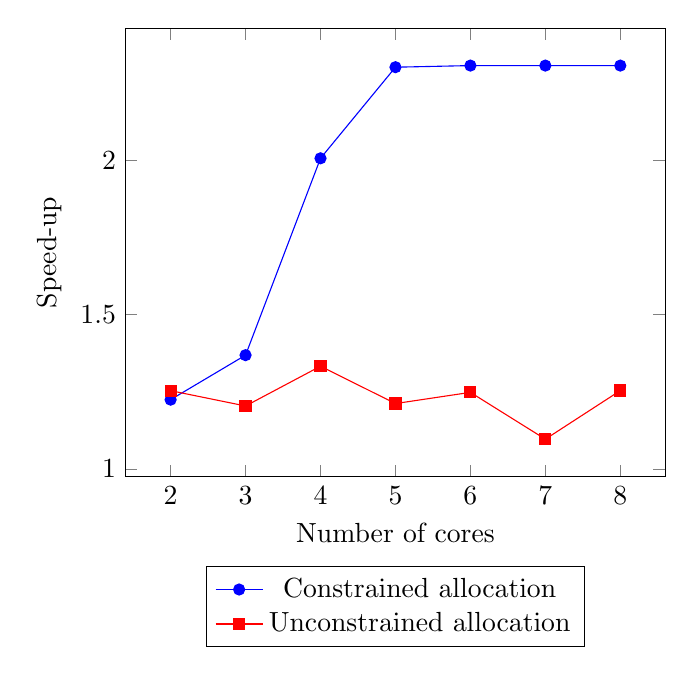
\begin{tikzpicture}
    \begin{axis}[
        xlabel=Number of cores,
        ylabel=Speed-up,legend style={at={(0.5,-0.2)},anchor=north}]
    \addplot[mark=*,blue,label=const] plot coordinates {
        (2,     1.223967163)
        (3,    1.368187328)
        (4,    2.005976773)
        (5,   2.301174325)
        (6,   2.306397786)
        (7,   2.306397786)
        (8,  2.306397786)
    };
    \addlegendentry{Constrained allocation}

    \addplot[color=red,mark=square*,label=unconst]
        plot coordinates {
        (2,     1.253126949)
        (3,    1.203511837)
        (4,   1.332430943)
        (5,   1.211351319)
        (6,  1.247650948)
        (7,  1.095957175)
        (8,  1.253420685)
        }; 
    \addlegendentry{Unconstrained allocation}
    \end{axis}
\end{tikzpicture}

\end{document}